\documentclass[border=6pt]{standalone}
\usepackage{tikz}
\usetikzlibrary{arrows.meta,calc,positioning}
\begin{document}
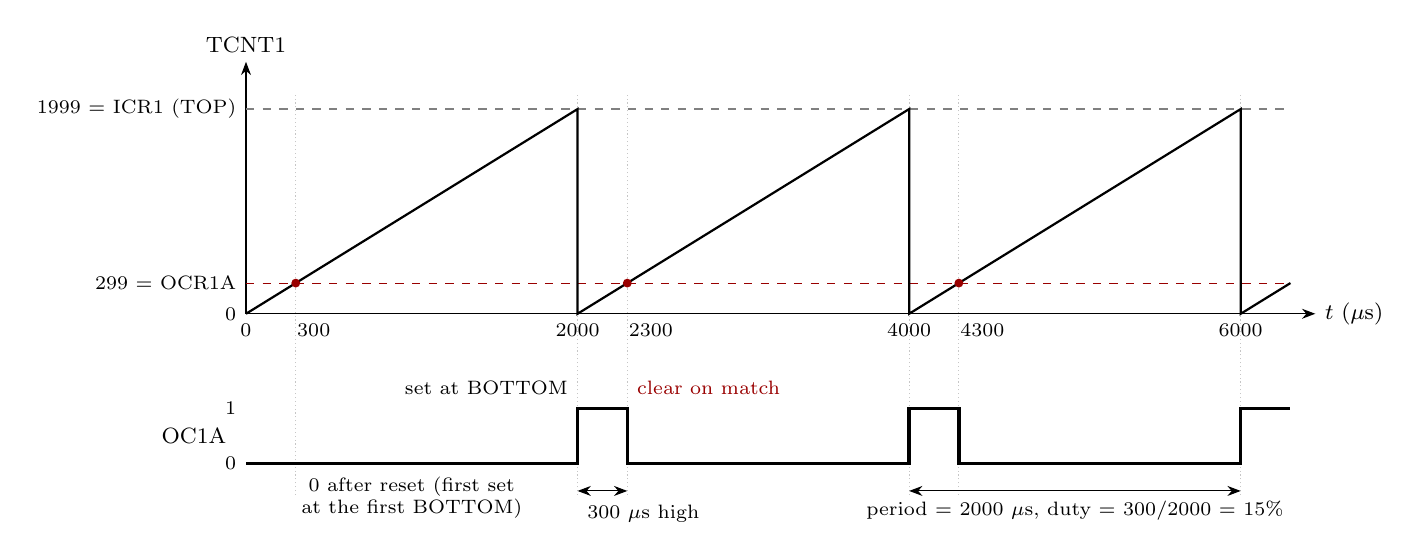
\begin{tikzpicture}[>=Stealth,font=\small,x=0.0021cm,y=1cm]
% 1 unit = 1 us; 1 tick = 1 us; period = ICR1 + 1 = 2000 ticks; OC1A high for OCR1A + 1 = 300 ticks
\def\H{2.6}% 1999
\def\C{0.3897}% 299 -> 2.6*299/1999
\foreach \t in {300,2000,2300,4000,4300,6000} \draw[gray!45,densely dotted] (\t,-2.3) -- (\t,\H+0.2);
\draw[->] (0,0) -- (0,\H+0.6) node[above,font=\footnotesize]{TCNT1};
\draw[->] (0,0) -- (6450,0) node[right,font=\footnotesize]{$t$ ($\mu$s)};
\node[anchor=east,font=\scriptsize] at (0,\H) {1999 = ICR1 (TOP)};
\node[anchor=east,font=\scriptsize] at (0,\C) {299 = OCR1A};
\node[anchor=east,font=\scriptsize] at (0,0) {0};
\draw[gray,dashed] (0,\H) -- (6300,\H);
\draw[red!60!black,dashed] (0,\C) -- (6300,\C);
\draw[thick] (0,0) \foreach \k in {1,2,3} { -- (\k*2000,\H) -- (\k*2000,0) } -- (6300,{\H*300/2000});
\foreach \k in {0,1,2} \fill[red!60!black] (\k*2000+300,\C) circle (1.6pt);
\foreach \t in {0,2000,4000,6000} \node[below,font=\scriptsize] at (\t,0) {\t};
\foreach \t in {300,2300,4300} \node[below right=0pt and -3pt,font=\scriptsize] at (\t,0) {\t};
% OC1A
\begin{scope}[yshift=-1.9cm]
\node[anchor=east,font=\footnotesize] at (-60,0.35) {OC1A};
\node[anchor=east,font=\scriptsize] at (0,0.7) {1};
\node[anchor=east,font=\scriptsize] at (0,0) {0};
\draw[very thick] (0,0) -- (2000,0) -- (2000,0.7) \foreach \k in {1,2} { -- (\k*2000+300,0.7) -- (\k*2000+300,0) -- (\k*2000+2000,0) -- (\k*2000+2000,0.7) } -- (6300,0.7);
\node[font=\scriptsize,red!60!black,anchor=south west] at (2300,0.75) {clear on match};
\node[font=\scriptsize,anchor=north,align=center] at (1000,-0.05) {0 after reset (first set\\at the first BOTTOM)};
\node[font=\scriptsize,anchor=south east] at (2000,0.75) {set at BOTTOM};
\draw[<->] (2000,-0.35) -- (2300,-0.35);
\node[font=\scriptsize,anchor=north west] at (2000,-0.4) {300 $\mu$s high};
\draw[<->] (4000,-0.35) -- (6000,-0.35) node[midway,below,font=\scriptsize]{period = 2000 $\mu$s, duty = 300/2000 = 15\%};
\end{scope}
\end{tikzpicture}
\end{document}
